\documentclass[./dissertation.tex]{subfiles}
\usepackage{amsfonts}
\begin{document}


    \contentchapter{Metric Learning}
    
    \section{Metric Learning as Representation Learning}
    It is a paramount for almost all tasks within the field of machine learning to build meaningful representations of the data. For instance, a representation of data is required for regression, classification, and clustering tasks. Multilayer perceptons model and other neural network models create successive representations of the input data before producing the output. Bengio defines representation learning as "learning representations of the data that make it easier to extract useful information when building classifiers or other predictors." \cite{bengio2013representation}\\
    
    Metric learning can thus be thought of as a type of representation learning, as in metric learning an embedding space is learned where similar samples are close together and dissimilar samples are far apart. The representation of data in a metric learning system is the latent representation of the data points. 
    \section{Metric Learning Overview}
    Metric learning attempts to create representations for data by training against the similarity or dissimilarity of samples. In a more technical sense, there are two notable functions in a metric learning system. Function $f$ is a neural network which maps the input data $X$ to the latent points $Z$ (i.e. $f_{\theta}: X \mapsto Z$, where $\theta$ is the network parameters). Generally, $Z$ exists in a space of much lower dimensionality than $X$ (eg. $X$ is a set of 28x28 pixel pictures and $Z \in \mathbb{R}^{10}$).\\
    
    The function $D(f_{\theta}(x_{1}), f_{\theta}(x_{2}))$ represents the distance between two inputs $x_{1}, x_{2} \in X$. To create a useful embedding model $f_{\theta}$, we would like for $f_{\theta}$ to produce large values of $D(f_{\theta}(x_{1}), f_{\theta}(x_{2}))$ when $x_{1}$ and $x_{2}$ are dissimilar and for $f_{\theta}$ to produce small values of $D(f_{\theta}(x_{1}), f_{\theta}(x_{2}))$ when $x_{1}$ and $x_{2}$ are similar.\
    
    It is common for the $l_{2}$ metric to be used as a distance function in metric learning. The generalized $l_p$ metric can be defined as follows, where $z_{0}, z{1} \in \mathcal{R}^{d}$.
          \begin{equation*}
            D(z_{0}, z_{1})= || z_{0} - z_{1} ||_{p} =
            (\sum_{i=1}^d | z_{0} - z_{1} |^{p})^{1/p} 
          \end{equation*}
    
    As the architecture of $f_{\theta}$ (a neural network) and the distance function $D$ (the $l_{2}$ metric) have been standardized, the most important remaining component in a metric learning system is the loss function for training $f$. The following section provides a survey of the development of and differences between notable training objectives in metric learning, which for brevity we will refer to as \textit{metric loss functions} or \textit{metric losses}.
    
    \section{Survey of Metric Loss Functions}
    
    \subsection{Contrastive Metric Losses}
    Contrastive metric losses encourage samples $x_{1}, x_{2}$ to have a small value $D(f_{\theta}(x_{1}), f_{\theta}(x_{2}))$ if $y_1 \eq y_2$ and for  $D(f_{\theta}(x_{1}), f_{\theta}(x_{2}))$ to have a large value if $y_1 \neq y_2$. In other words, contrastive metric losses encourage similar samples or samples of the same class to be close together or dissimilar samples or samples of different classes to be far apart. It may seem confusing at this stage how this goal of \textit{contrastive} metric losses is distinct from the goal of metric learning more generally. This makes more sense in relation to class-based metric losses, ... \\
    
    One of the first contrastive metric losses is contrastive loss \cite{chopra2005learning}. Contrastive loss minimizes the distance between a pair of points $f_{\theta}(x_{1}), f_{\theta}(x_{2})$ if they are of the same class and maximizes the distance if the points are of different class. \\ 
    \begin{equation*}
            L_{contrastive}(\theta, x_{1}, x_{2}, y_{1}, y_{2})
            = 1_{y_{1} = y_{2}}L_{G}(D(f_{\theta}(x_{1}), f_{\theta}(x_{2})))
            + 1_{y_{1} \neq y_{2}}L_{I}(D(f_{\theta}(x_{1}), f_{\theta}(x_{2})))
    \end{equation*}
    In this objective function, $L_{G}$ refers to the loss function for "genuine pairs" of the same class, $L_{I}$ refers to the loss function for "imposter pairs" of different classes, and $1_{b}$ is a piecewise function that is 1 if $b$ is true and 0 if $b$ is false. One common instantiation of these loss functions is the following \cite{weng2021contrastive}.
    \begin{equation*}
            L_{G}(D) = D \\
    \end{equation*}  
        \begin{equation*}
            L_{I}(D) = max(0, \alpha - D) 
    \end{equation*}  
    In this instantiation, $L_{G}$ is simply the identity function, or the raw distance, and $L_{I}$ is the distance subtracted from a hyperparameter $\alpha$ and constrained by a lower bound of 0. This effectively bounds the partial loss function for \_ pairs. Intuitively, the function looks to minimize distance between embeddings of in similar pairs and maximize distance between embeddings in dissimilar pairs. \\
    
    Triplet loss is another simple contrastive metric loss and perhaps the most popular loss used in metric learning today. Triplet loss is originally proposed as follows \cite{schroff2015facenet}. 
    \begin{equation*}
    L_{contrastive}(\theta, x_{a}, x_{p}, x_{n}) =
    |D(f_{\theta}(x_{a}), f_{\theta}(x_{p})) - D(f_{\theta}(x_{a}), f_{\theta}(x_{n})) + \alpha|
    \end{equation*} 
    
    In this loss objective, $x_{a}$ is an anchor point, $x_{p}$ is a positive sample (of the same class as the anchor point), and  $x_{n}$ is a negative sample (of a different class than the anchor point). These three points constitute a triplet in triplet loss. In the original paper, the authors note that "hard triplets", or triplets in which the distance between positive samples $D(f_{\theta}(x_{a}), f_{\theta}(x_{p}))$ exceeds or is within a certain bound $\alpha$ of the distance between negative samples $D(f_{\theta}(x_{a}), f_{\theta}(x_{n}))$ are especially crucial for training. 
    
    \begin{figure}[h]
        \centering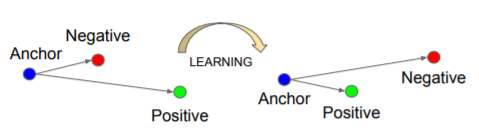
\includegraphics[width=0.5\textwidth]{figures/triplet_loss_figure}
        \caption{Diagram of the relative distances between triplet points. The distance between the anchor and the positive point should be minimized and the distance between the anchor and the negative point should be maximized. (Source: Schroff et al., 2015)}
        \label{Triplet Loss Diagram}
    \end{figure}
    
    The N-pair loss \cite{sohn2016improved} extends on triplet loss to include more than one negative sample for each anchor and positive sample pairing. The authors write that by only comparing the anchor against one negative sample per loss computation, it takes much longer for the loss to converge. The N-pair is especially useful for datasets in which there is more than two classes, as it would follow that there are more negative samples than positive samples for each point. Consider a tuple of $n + 1$ element consisting of an anchor point $x_{a}$, a positive sample $x_{p}$, and $i$ negative samples $x_{n}^{1}, x_{n}^{2}, ..., x_{n}^{i}$. We can then define the loss objective as follows.
    \begin{equation*}
    L_{N-pairs}(\theta, x_{a}, x_{p}, x_{n}^{1}, x_{n}^{2}, ..., x_{n}^{N - 1}) = log(1 + \sum_{i=1}^{N-1} 
    exp(f_{\theta}(x)^{T} f_{\theta}(x_{n}^{i}) 
    - f_{\theta}(x)^{T} f_{\theta}(x_{p})
    )
    \end{equation*} 
    The N-pair loss differs from triplet loss primaily not only in the use of multiple negative samples but in it's use of the inner-product in the place of a distance metric. In this sense, the N-pair loss is very similar to a softmax loss.
    
    There are several problems with contrastive approaches generally that have recently caused researchers to move away from contrastive approaches \cite{hav4ik2021deepmetriclearning}. One of these issues is the computational complexity of sample mining. For most contrastive approaches, take triplet loss for example, the most difficult triplets (in terms of minimizing the loss function) should be mined for the model to converge quickly. However, finding such triplets is often computationally expensive. Another issue with contrastive approaches is that the metric losses do not necessarily cause similar labels to cluster together in the same regions at a global level. Both of these issues are addressed by more recent metric loss functions.
    
    \subsection{Modern Metric Losses}
    Modern metric loss functions address the shortcomings of traditional contrastive metric losses, such as supervised contrastive loss \cite{khosla2020supervised}. Supervised contrastive loss further generalizes triplet and N-pair loss by using many positive and many negative samples for each loss computation, which the authors attribute as the reason the loss is able to converge quickly without mining for hard samples. \\ 
    
    \begin{equation*}
    L_{out}^{sup} = \sum_{i \in I} \frac{-1}{|P(i)|}
    \sum_{p \in P(i)}log(\frac{exp(z_{i} \cdot z_{p} / \tau)}
    {\sum_{a \in A(i)}exp(z_{i} \cdot z_{a} / \tau)}) 
    \end{equation*} 
    \begin{equation*}
    L_{in}^{sup} = \sum_{i \in I} -log(\frac{1}{|P(i)|}\sum_{p \in P(i)}
    \frac{exp(z_{i} \cdot z_{p} / \tau)}
    {\sum_{a \in A(i)}exp(z_{i} \cdot z_{a} / \tau)}) 
    \end{equation*}
    
    The two implementations proposed in the paper differ only in the summation being outside or inside the logarithm. In both equations, $I = {1, ..., 2N}$ is the set of indexes in the batch, $A(i) = I \\ i$ is the set of indexes excluding $i$, $P(i) = (p \in A(i) : y_{p} = y _{i})$ is the set of positive indexes in the batch for a given index $i$ excluding $i$ itself, and $\tau \in \mathcal{R}^{+}$ is a temperature hyperparameter. Like the N-pair loss, the supervised contrastive loss is modeled around the softmax loss. Unlike the N-pair loss, the supervised contrastive loss can be computed once per batch and accommodates multiple positive samples in one computation. \\
    
    The center loss is another important modern metric loss in solving some of the problems with contrasting learning. \cite{10.1007/978-3-319-46478-7_31}. To address the aforementioned problem of latent points not self-organizing into regions based on class, the authors introduce a center loss $L_{C}$ to encourage a point of class $y_{i}$ to be close to the corresponding class center. The class center $c_{y_{i}}$ for class $y_{i}$ is a trainable parameter which updates with the overall loss function, which is stated below.
    \begin{equation*}
    L_{C} = \frac{1}{2}\sum_{i = 1}^{m}||x_{i} - c_{y_{i}}||_{2} \end{equation*}
    \begin{equation*}
    L_{S} = - \sum_{i = 1}^{m}\frac{exp(g_{y_{i}}(x_{i}))}{\sum_{j = 1}^{n}exp(g_{j}(x_{i}))} 
    \end{equation*}
    \begin{equation*}
    L = L_{S} + L_{C}
    \end{equation*}
    As evident from the above equations, the center $L_{C}$ is added to a softmax loss $L_{S}$ in the overall loss function. $g_{c}$ refers to the classification layer of the softmax with the weights and bias of class $c$, and $m$ and $n$ are the number of classes and samples in the batch, respectively. \\
    
    Center loss can be viewed as one of the first steps in many of today's state of the art metric learning objectives. The SphereFace loss \cite{liu2017sphereface} is largely a modification of center loss's softmax function. SphereFace normalizes the class centers to be points on a hypersphere which provides a gurantee for inter-class variability. This is accomplisehd through normalizing of each row of the weight's matrix in the softmax function such that the norm of the row vector is 1. SphereFace additionally adds a margin term such that the decision boundary between classification of a point with softmax is more robust.  Other State-of-the-Art metric losses, such as CosFace \cite{wang2018cosface}, ArcFace \cite{deng2019arcface}, and AdaCos \cite{zhang2019adacos} are largely inspired by SphereFace and further explore the idea of a margin term for a decision boundary in the realm of angular projection \cite{hav4ik2021deepmetriclearning}. 
\end{document}
